\documentclass{article}
\usepackage[utf8]{inputenc}
\usepackage{graphicx}

\title{BDSA00}
\author{anjp }
\date{September 2021}

\begin{document}

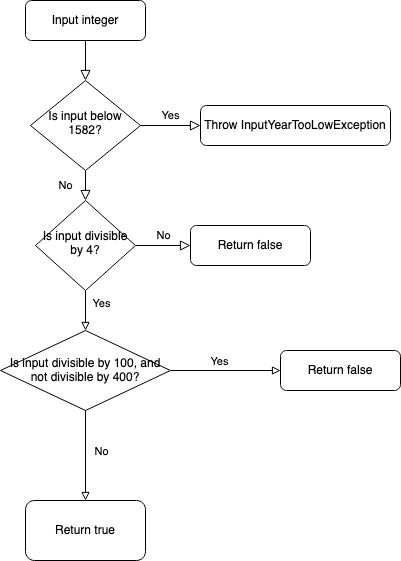
\includegraphics[height=10cm]{IsLeapYearFlow.drawio.png}
\\\\
The image is a flowchart with the decisions the algorithm makes. \\
The algorithm takes an integer as input. It then checks to see if the input is a number lower than 1582. If it is lower than 1582, it throws an \texttt{InputYearTooLowException}.
If it is not below 1582, the algorithm continues and checks to see if the input is divisible by 4. If it is not, it returns false, otherwise is checks if the input is divisible by 100 and not divisible by 400. It that is true, it returns false, otherwise it returns true.
\end{document}
